\documentclass[a4paper,zihao=5,UTF8]{ctexart}
\usepackage[top=2.3cm,bottom=2cm,left=1.7cm,right=1.7cm]{geometry} 
\usepackage{amsmath, amssymb}
\usepackage{color}
\usepackage{hyperref} 
\usepackage{pythonhighlight}
\usepackage{listings}
\usepackage{mathrsfs} 
\usepackage{booktabs}
\usepackage{amsthm}
\usepackage{longtable} 
\usepackage{graphicx}
\usepackage{subfigure}
\usepackage{caption}
\usepackage{fontspec}
\usepackage{titlesec}
\usepackage{fancyhdr}
\usepackage{latexsym}
\usepackage{subfigure}
\usepackage{braket}
\usepackage{cite}
\usepackage[version=4]{mhchem}

\CTEXsetup[format={\Large\bfseries}]{section}
\def\d{\mathrm{d}}
\def\e{\mathrm{e}}
\def\i{\mathrm{i}}
\def\dps{\displaystyle}
\newcommand{\mr}[1]{\mathrm{#1}}
\newcommand{\mb}[1]{\mathbf{#1}}
\newcommand{\dv}[2]{\frac{\d{#1}}{\d{#2}}}
\newcommand{\pdv}[2]{\frac{\partial{#1}}{\partial{#2}}}
\def\degree{$^{\circ}$}
\def\celsius{$^{\circ}\mr{C}$}
\title{\textbf{实验一 \ce{SrO}-\ce{Al2O3}二元体系中几种荧光材料的合成和表征\cite{inorganic_chemistry_1}}}
\author{王崇斌\;1800011716}
\makeatletter
\makeatother
\begin{document}
	\pagestyle{fancy}
	\pagestyle{fancy}
    \lhead{无机化学实验}
	\chead{}
	\rhead{\today}
	\maketitle
    \thispagestyle{fancy}
	\section{实验目的}
	\begin{enumerate}
		\item 学习高温固相合成的基本方法
		\item 学习软化学制备前驱体的基本方法
		\item 了解固体荧光材料的发光原理和基本表征方法
	\end{enumerate}
	\section{实验原理}
	\subsection{高温固相合成}
	高温固相合成通常用于合成无机固体材料。反应中存在多个固体物相,反应主要
	发生在固态反应物的接触面上,同时在其上形成产物层;然后反应物通过扩散作用跨过产物层
	进一步反应。由于固相难以混合充分,反应物颗粒之间的接触面积大小受反应物颗粒直径影响明显
	,同时由于固体中原子扩散速率远低于液相或气相(晶格比较稳定,常温下只会在平衡位置
	附近振动),因此固相化学反应通常需要在高温下进行(增加固体中原子的扩散速率,甚至
	熔化反应物或者产物以达到充分混合的目的),反应时间较长,难以得到高纯度、均匀的、物相单一
	的产物。
	\par 
	通常影响固相化学反应速率的因素都有:反应温度(这个前面讨论了),反应物混合的均匀程度(决定了
	反应物之间的接触面积),反应物物相(不同的物相有着不同的表面能和稳定性),添加助溶剂(提高
	反应物表面离子的扩散速率),等等。
	\subsection{软化学制备前驱体}
	除了机械研磨之外,还可以针对不同的反应体系设计出利用化学反应来充分混合反应物的方法,这个
	过程称为软化学制备反应前驱体。其主要的思路是利用水溶液稳定均一的特性,从溶液中
	想办法“提取”出固态的前驱体,这就需要利用反应物的化学性质来设计制备前驱体的反应。
	通常使用的方法有\textbf{共沉淀法}、\textbf{溶胶凝胶法}、\textbf{燃烧法}。
	在本实验中使用了燃烧法。
	\par 共沉淀法是指在均相溶液中加入沉淀剂,使多种阳离子以\textbf{共晶}的方式沉淀下来,理想
	情况下共沉淀物可以达到原子量级的混合程度,混合效果远高于机械研磨法。
	但是由于不同物种溶度积不同,很有可能发生偏析——即某个物种优先沉淀的现象,
	从而导致混合并不均匀。因此沉淀剂的选择和沉淀条件(ph、温度等)的控制就显得尤为重要。
	溶胶凝胶法利用金属醇盐的缓慢水解,然后逐渐缩聚最终生成凝胶的过程将阳离子充分混合。燃烧法
	通常是在金属硝酸盐溶液中加入还原剂,加热浓缩,而后升高温度让硝酸根与还原剂发生激烈的氧化
	还原反应,可以在较短的时间内获得混合充分的金属氧化物混合物。通常加入的还原剂是含有羟基的
	羧酸比如柠檬酸或者甘氨酸和尿素这类能够起到一定螯合作用的还原剂。
	\subsection{荧光材料的发光原理}
	荧光材料一般由\textbf{基质}和\textbf{激活剂}组成。基质材料通常是由满壳层离子构成的稳定
	固体化合物,禁带较宽,在可见光范围内没有吸收;激活剂是不满壳层的离子,以固溶形式溶解在基
	质中,电子在壳层内或邻近壳层之间跃迁产生吸收和荧光发射。\ce{SrO-Al2O3}二元体系中几种
	不同Sr-Al比例的铝酸锶相均是优良的基质材料,\ce{Eu^{2+}}可以作为该基质中的优良激活剂。
	\ce{Eu^{2+}}的激发过程为$4f^7\to4f^ 65d ^1$的$d-f$跃迁,其中$f$电子构成受配位环境
	影响较小的窄能级,$5d$轨道受配位场影响较为明显。因此\ce{Eu^{2+}}周围的配位场越强,$d$
	轨道分裂越大,导致$d$轨道形成的能带下沿降低,因此基质的组成(在本实验中表现为\ce{Sr}与\ce{Al}
	)明显影响着其中\ce{Eu^{2+}}的发光行为。
	\par 
	如果进一步在这样的晶体中掺入\textbf{陷阱离子},有可能得到\textbf{长余辉材料}。\ce{Dy ^{3+}}
	是一种合适的陷阱离子,在紫外光或者可见光激发下,激活剂离子\ce{Eu^{2+}}从基态跃迁到激发态(
	上一段中描述过的$d-f$跃迁),部分激发态电子直接跃迁至基态发出波长$\approx 520\mr{nm}$的
	绿色荧光;另一部分激发态电子在热微扰下进入导带,随后被\ce{Dy^{3+}}形成的陷阱能级
	捕获(这个中心含有\ce{Dy^{3+}}因此有吸引电子的倾向),同时将能量储存在该激发态能级中。当
	此激发态收到热微扰时,将电子释放回导带,并通过\ce{Eu^{2+}}的激发态跃迁回基态,同时发出荧光。
	\section{实验操作步骤}
	实验地点:北京大学化学院D区3楼第一教学实验室2号实验台
	\par 
	实验时间:2021年3月26日(星期五)
	\subsection{高温固相反应合成荧光材料}
	实验者被分配到S2组,目标合成物为\ce{Sr_{3.84}Al_{14}O_{25}}:0.04\ce{Eu^{2+}},0.08\ce{Dy^{3+}}。
	\par 
	称取
	\footnote{括号前为理论需要量,括号中为实际称取量}
	1.3338g(1.3333g)\ce{SrCO_{3}},2.1841g(2.1835g)\ce{Al(OH)_{3}},0.0141g(0.0147g)\ce{Eu_2O_3}
	,0.0298g(0.0314g)\ce{Dy_2O_3},\\0.1008g(0.1008g)\ce{H_3BO_3},
	将这些固体粉末放置于玛瑙研钵中,加入少量无水乙醇使体系呈现出粘稠状,用力研磨15分钟(研磨是否
	充分直接决定了产物的质量),避免原料溅出。
	\par
	将上述研磨过的粉末装入氧化铝坩埚,墩实,在样品表面放上几根碳棒
	\footnote{注意!实验室中有两种碳棒,一种表面光滑不易掉渣(看起来更像石磨棒),另一种
	颜色更黑容易掉渣,不要将容易掉渣的碳棒放入坩埚中,否则产物表面回沾上难以去除的碳,使
	产物色泽变差。这是实验者实验中遇到的问题。},盖上坩埚盖后放入大坩埚中,加入碳棒后盖上
	套埚盖,移入马弗炉快速升温至$\approx 1300$\celsius,恒温2小时,降温至1000\celsius
	后出炉,冷却至室温将样品取出,可以明显观察到产物为淡黄绿色块状,与放入的反应物
	形状有很明显不同。
	\par 
	去除样品表面的碳棒,同时刮去粘在样品上的碳粉,将样品转移到玛瑙研钵中,盖好防溅有机玻璃板,
	将样品敲碎研细,分出一少半装入自封袋。
	\subsection{燃烧法合成荧光材料前驱体}
	目标:合成0.01\ce{mol}\ce{Sr_{0.96}Al_{2}O_{4}}:\ce{0.01Eu^{2+}},\ce{0.02Dy^{3+}}
	荧光材料前驱体
	\paragraph{配置A溶液}
	称取\footnote{括号内为实际使用量}
	2.03g(2.0303g)\ce{Sr(NO_3)_2},7.50g(7.5104g)\ce{Al(OH)_3*9H_2O},0.03g(0.0329g)\ce{Eu(NO_3)_3}\\
	0.09g(0.0914g)\ce{Dy(NO_3)_3},40-50mg(0.0430g)\ce{H_3BO_3},放入\textbf{石英烧杯}
	\footnote{注意区分石英烧杯和普通的烧杯}
	中,加入12ml去离子水,磁力加热搅拌至完全溶解。
	\paragraph{配置B溶液}
	称取5.40g(5.40g)尿素,加入6ml去离子水,磁力加热搅拌至溶液澄清。
	\paragraph{制备凝胶}
	将B溶液加入A溶液中,加热搅拌下蒸发一定水分,前驱体浓缩至粘稠半透明凝胶时(注意
	快蒸干时会观察到溶液剧烈产生气泡,一定要在这个阶段之前停止加热,否则在冷却时溶液固化
	导致磁子难以取出)取出磁子停止加热。
	\paragraph{凝胶燃烧}
	擦干石英烧杯外侧的水渍,将其移入已预热的500摄氏度热解炉中,前驱体会在其中沸腾起泡,
	泡沫状的前驱体将充满整个烧杯,当水快要蒸干时可以看到有淡黄色气体放出,同时前驱体会从内而外
	燃烧,放出红黄色火焰,持续时间较短。燃烧结束后产生白色疏松产物(此时还可以观察到有
	蒸汽产生),盖上恒温盖恒温10min后取出,冷却回收。
	\section{荧光材料的表征}
	\subsection{发光性能的表征}
	表征仪器:Nanolog红外荧光测试系统
	\par
	将样品测试架(铜制)放在平板玻璃上,使样品架紧贴玻璃。将研细的样品粉末倒入凹槽,
	用压紧棒将样品间的空气排出,再用力将样品压实,压紧后在样品背面贴上黑胶布避光,
	正面贴上盖玻片保护。翻转检查,样品面应于样品架平面齐平。
	\par
	发光光谱测试条件:根据样品选择合适的激发波长和发射波长记录范围。
	数据采集间隔1 nm;激发狭缝5 nm;发射狭缝0.5 nm;积分时间0.1 s。
	测试在激发150s达到饱和后进行。
	\par
	储能余辉衰减曲线测试条件:根据样品选择合适的激发波长和发射波长记录范围。
	数据采集间隔0.1 s;激发狭缝1.1 nm;发射狭缝3.0 nm;测试时间范围:0.1-300s,在测试
	进行150s后激发饱和时停止激发,测试余晖衰减曲线。
	\subsection{物相的鉴定}
	表征仪器:岛津XRD-600
	\par
	将样品框放在平板玻璃上,使样品框紧贴玻璃。将研细的样品粉末倒入凹槽中,用另一块载玻片将样品压实。
	翻转检查,样品面应于样品架平面齐平,竖直样品框时样品不掉落。
	测试条件:铜靶,Ni滤波器,X射线管电压/电流:40 kV/20 mA,扫描速度5°/分,2θ扫描范围19.5° ~ 32.5°。
	发射狭缝(DS):D1-1.7 mm,防散射狭缝(SS):S1-0.6 mm,接收狭缝(RS):0.3 mm。
	\section{实验结果讨论}
	\subsection{发光性能分析}
	表格\ref{table of fluorescence}给出了S2组产物荧光的基本数据,图\ref{S2 fluorescence spectrum}
	展示了S2小组的各个样品的发射光谱,可以看出实验者制备的样品有着较好的荧光效果,如果在烧制时
	选择质量好的碳棒,减少样品中吸附的碳,有可能会体现出更好的荧光性能。荧光性能较好的另一个原因
	可能与准备前驱物时研磨充分,准备的待检测样品表面比较平整有很大关系。
	\par 
	图\ref{S2 fluorescence residual}给出了储能和余辉衰减曲线。从表\ref{table of fluorescence}
	中数据可以看出发射强度和余辉的强度呈现出正相关
	。尝试了很久考虑通过指数衰减的函数来拟合余辉
	衰减的过程,但是效果不佳,可能的原因是余辉衰减速率远高于指数衰减的速率。但是能看到
	一个明显的趋势,所有样品的余辉衰减非常迅速,这与日常生活中遇到的长余辉材料很不相同,
	个人推测的结果是1.烧结的过程中时间略短,产物没有形成很好的晶相(晶体缺陷较多的话会影响
	荧光)2.制样的过程中研磨了产品,破坏了其中生成的晶体结构,长程有序的结构被破坏后会影响
	发光效率。
	\paragraph{产物的荧光相对强度}
	实验者制作S2,样品编号07,荧光绝对强度为164851(标准为172318),荧光相对强度为
	$95.7\%$。
	\paragraph{产物的余辉相对强度}
	实验者制作S2,样品编号07,余辉绝对强度为1590(标准为1700),余晖的相对强度为
	$93.5\%$。
	\begin{table}[htbp]
	\caption{S2样品的发光性能}%标题
	\centering%把表居中
	\begin{tabular}{cccccc}%四个c代表该表一共四列,内容全部居中
	\toprule%第一C道横线
	学号 & 编号 & 荧光绝对强度 & 荧光相对强度 & 余辉绝对强度 & 余辉相对强度 \\
	\midrule%第二道横线 
	1600011744 & 01 & 123641 & $71.7\%$ & 1210 & $71.2\%$ \\
	1800011784 & 05	& 152989 & $88.8\%$ & 1860 & $109.4\%$ \\
	1800011836 & 06 & 172318 & $100\%$ & 1700 & $100\%$ \\
	1800011716 & 07 & 164851 & $95.7\%$ & 1590 & $93.\%5$ \\
	1900011758 & 09 & 110090 & $63.9\%$	& 950 & $55.9\%$ \\
	\bottomrule%第三道横线
	\end{tabular}
	\label{table of fluorescence}
	\end{table}
	\begin{figure}[htbp]
		\centering
		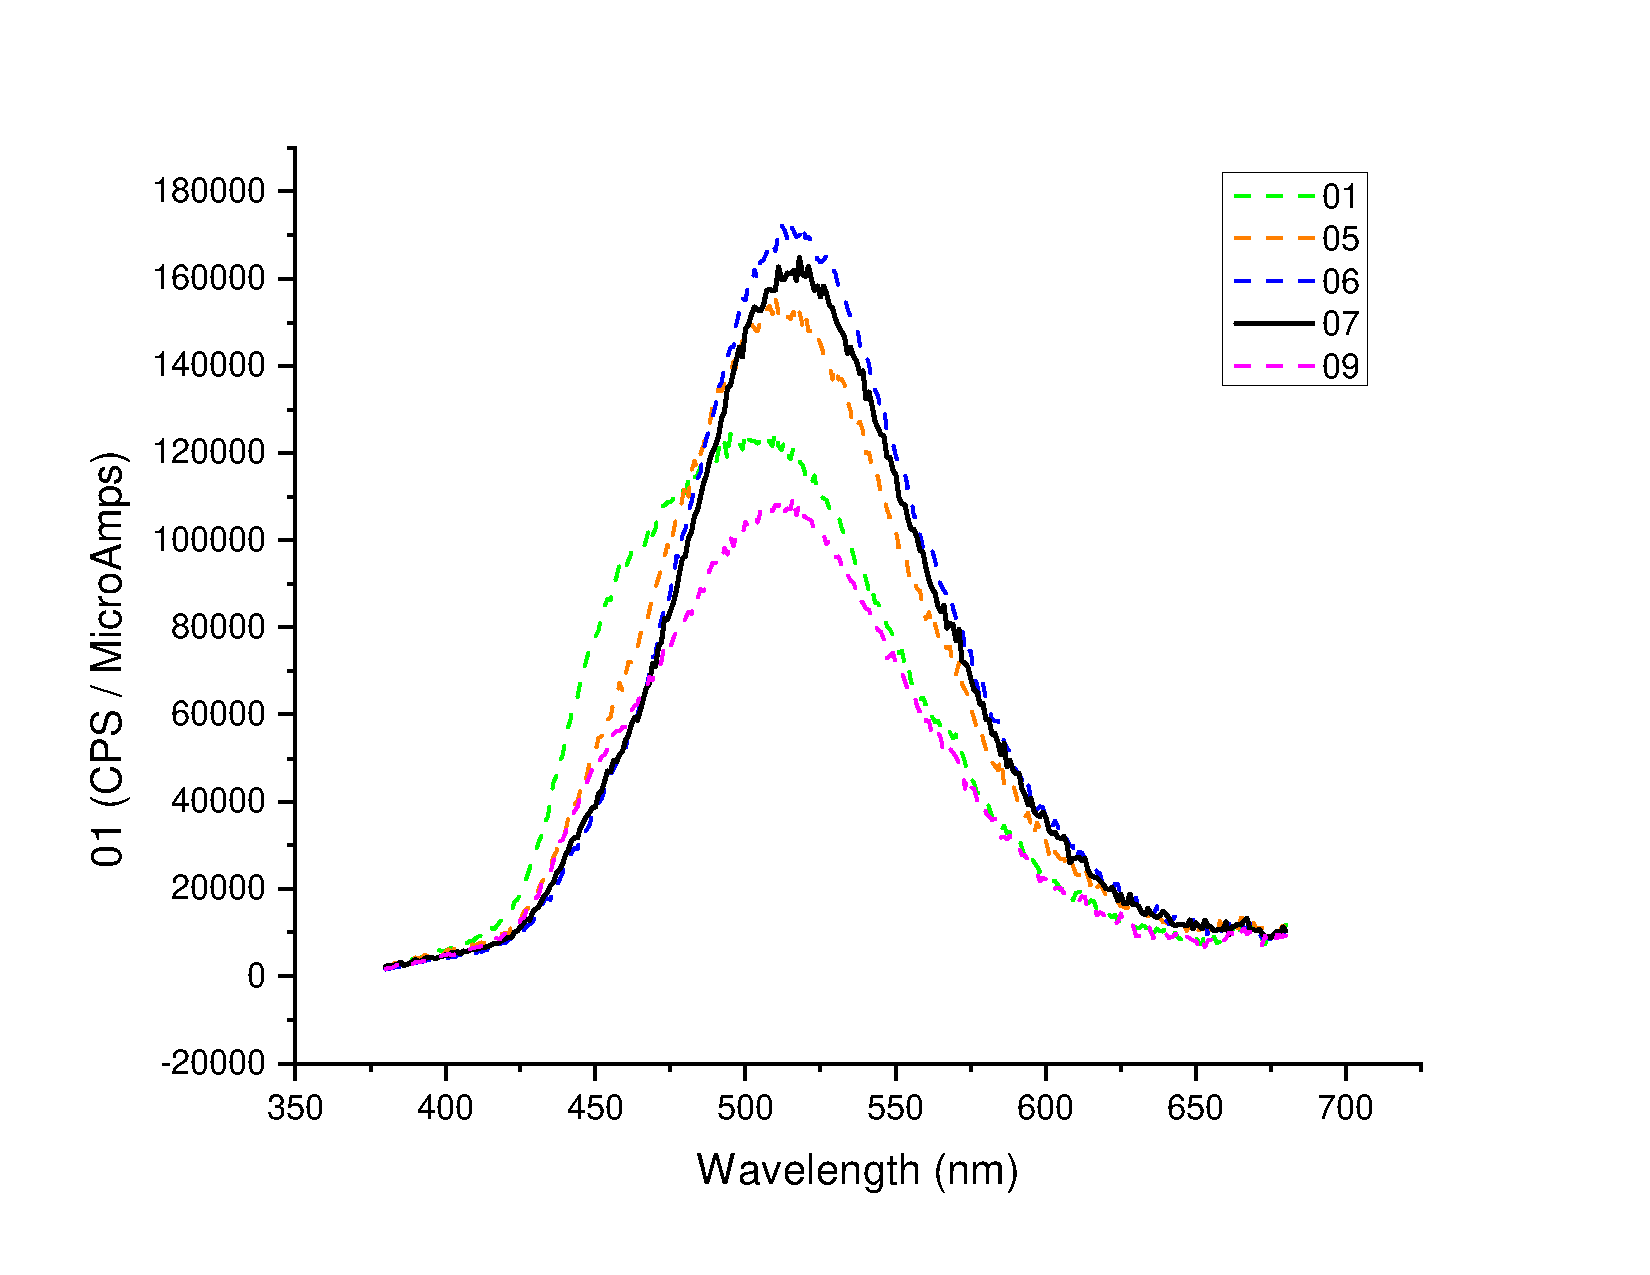
\includegraphics[scale=0.50]{S2fluorescence.pdf}
		\caption{S2小组样品的发射光谱}
		\label{S2 fluorescence spectrum}
	\end{figure}
	\begin{figure}[htbp]
		\centering
		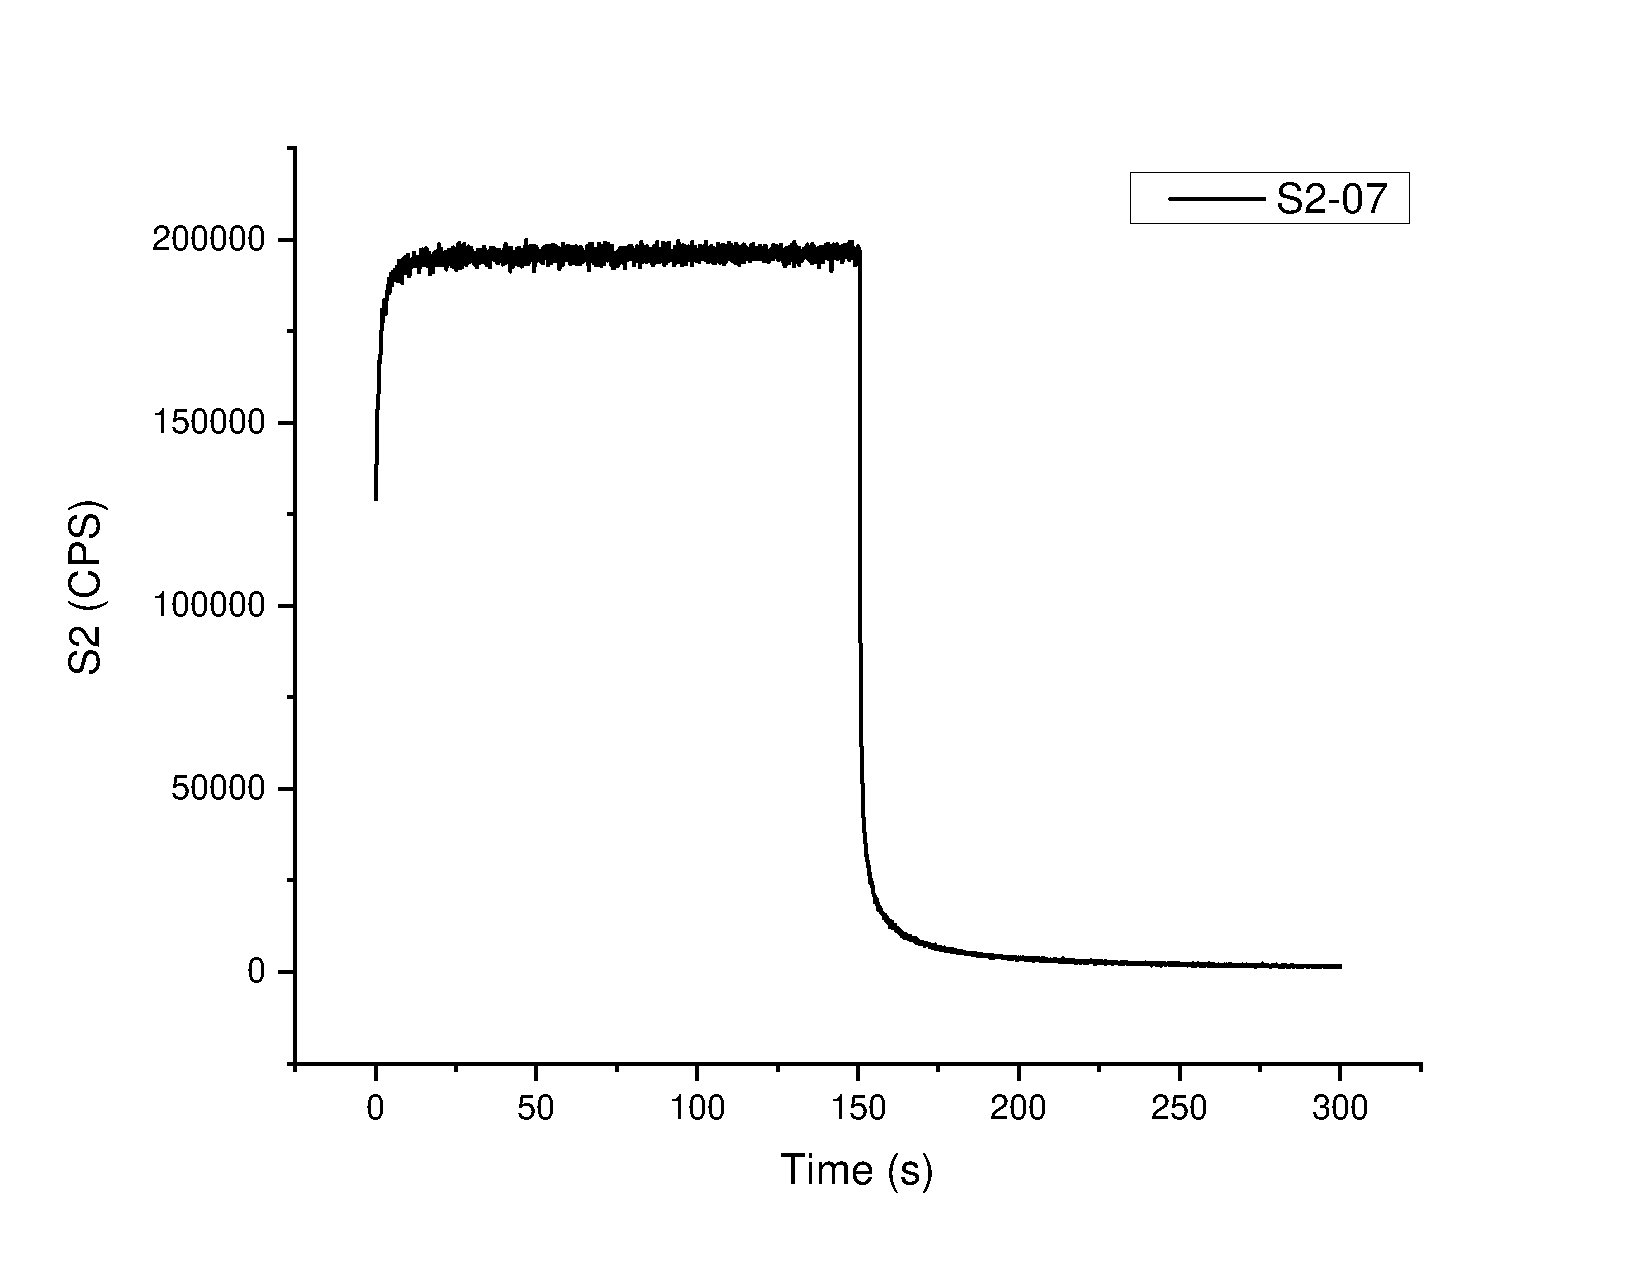
\includegraphics[scale=0.50]{S2residual.pdf}
		\caption{实验者样品的储能和余辉衰减曲线}
		\label{S2 fluorescence residual}
	\end{figure}
	\subsection{物相分析}
	\begin{figure}[htbp]
		\centering
		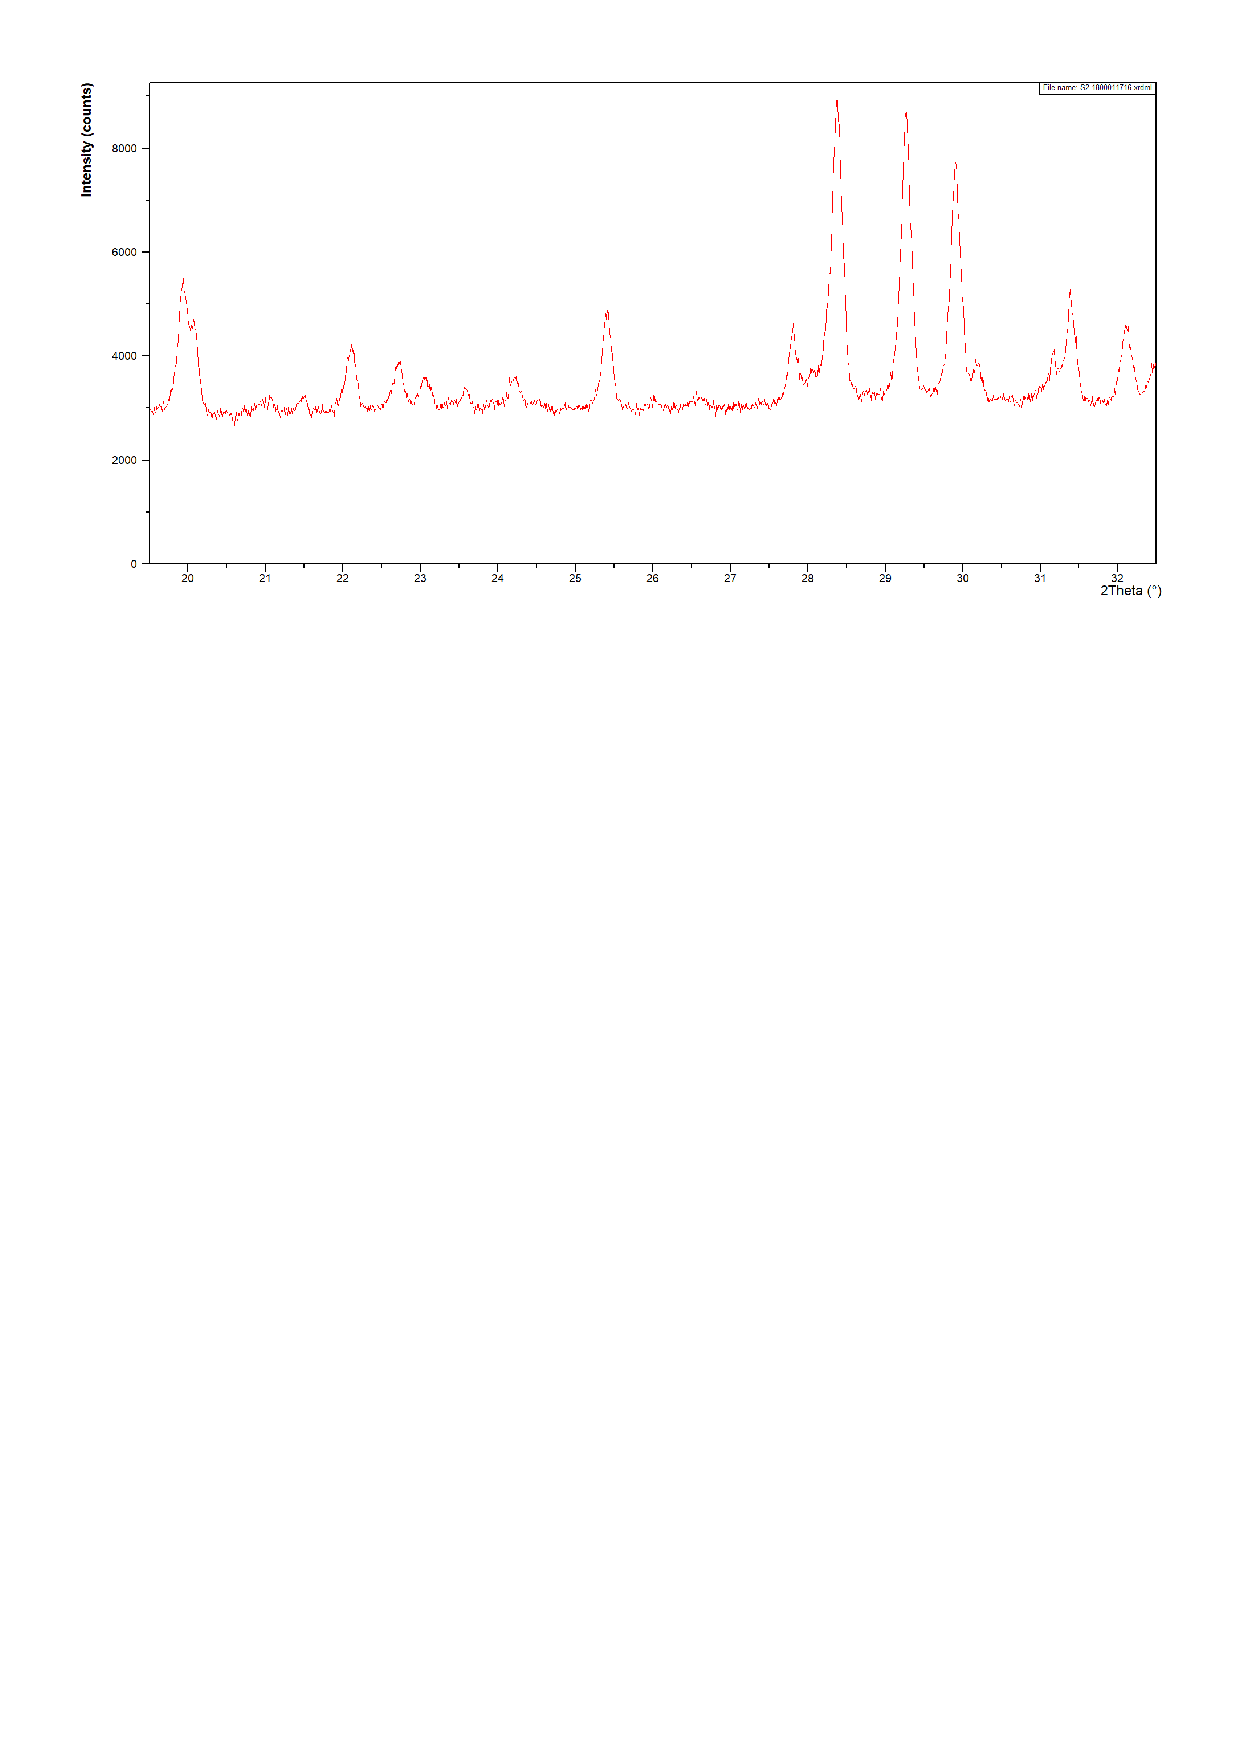
\includegraphics[scale=0.60]{S2-1800011716.pdf}
		\caption{实验者样品的XRD图谱}
		\label{S2 XRD}
	\end{figure}
	观察实验者样品的图谱\ref{S2 XRD},可以看到衍射角在28\degree - 30 \degree 处有三个明显的
	峰,对比标准谱图可知这有可能是\ce{SrAl_2O_4}和\ce{SrAl_4O_7}的衍射峰,但是对比25 \degree 
	附近的衍射峰可知,不可能是\ce{Sr_Al_4O_7}产生的衍射峰,只可能是\ce{SrAl_2O_4}产生的
	衍射峰,这同时给出了20 \degree 两侧衍射峰的来源
	。25 \degree 右侧的衍射峰是\ce{Sr_4Al_14O_25}产生的,同时观察28 \degree 左侧和31 \degree 右侧
	的小峰,可以印证\ce{Sr_4Al_14O_25}的存在。个人认为32 \degree 右侧的衍射峰是\ce{SrAl_12O_19}产生的。
	\par 
	对比31 \degree 右侧和30 \degree 左侧的衍射峰,容易判断\ce{SrAl_2O_4}是产物的主要成分,这与合成
	的目标相去甚远,主要产物是S1组的产物,这点也从荧光数据中得到了证实,两组的荧光光谱事实上
	没有明显的差异。这种普遍的情况可能说明了S2的合成方法有些问题。
	\section{思考题}
	\paragraph{1.}在平衡反应中,反应物和产物的浓度均不为零。这一说法对固相反应适用吗?
	固相化学反应和溶液化学反应有何不同?它们的完成程度受到什么规律的支配?
	\paragraph{答:}如果固相化学反应有机会进行到热力学平衡的阶段,就会受化学平衡规律支配,
	即反应物和产物浓度均不为零。固相化学反应由于固体物理性质的影响,反应物接触不充分、无法充分混合等
	导致反应在动力学上非常不利,因此固相化学反应主要受到动力学支配;而溶液中的化学反应由于溶液均一稳定的性质,一般来说可以得到充分地混合与接触,
	因此溶液中地反应主要受到热力学支配。
	\paragraph{2.}固相化学反应能够在室温下以较高的速率进行吗?需要什么条件?
	\paragraph{答:}由于动力学上的阻碍,希望固相反应在室温下快速进行的唯一方法就是通过机械研磨
	提供额外的能量。
	\paragraph{3.}什么是“非整比化合物”?其有什么特殊性质?本实验合成的产物是否属于非整比化合物?
	\paragraph{答:}非整比化合物指的是组成中各类原子的相对数目不能用几个小的整数比表示的化合物。
	其组成可以在较小范围内变化而不改变整体的结构,这给参杂其他金属离子提供了机会,我认为我们合成的
	材料属于非整比化合物。
	\bibliographystyle{plain}
	\bibliography{ref}
\end{document}